\documentclass{article}
\usepackage{geometry}
\geometry{margin=.5in}
\usepackage{amsmath}
\usepackage{mathtools}
%Figures and tables
\usepackage{float}
%Inserts images
\usepackage{graphicx}
%Linking
\usepackage{hyperref}
%Drawing
\usepackage{tikz}
\usetikzlibrary{angles, quotes}
%Includes "References" in the table of contents
\usepackage[nottoc]{tocbibind}

\newcommand{\norm}[2][]{\left\lVert#2\right\rVert_{#1}}

\title{AI Manifesto: a Non-TLDR Approach}

\author{Batuhan Karaca}

\numberwithin{equation}{subsection}
\begin{document}

\maketitle
\tableofcontents
\section{Introduction}
\subsection{Binding Information (TLDR)}
This book aims to give intuition for some ML (machine learning) concepts that I thought of significance. I started writing it simply because of the fact that I was bored of reading TLDR textbooks without understanding anything at all. That is why, I tried to give information as concise and as clear as possible. This compound thingy is solely my research and notetaking work piled up over years. I am trying to teach the topic using mostly mathematical proofs, though I also provide examples and/or explanations. I hope this book will be helpful for people wanting a career in the field.

I am not claiming to have 100\% accurate statements, though have I not seen any conflictions between my findings and the publications. I do not think any theory is perfect as well. They are good only because they just work in practice. Furthermore, I am not claiming this book to be a textbook material on its own. I only wanted to share (hopefully) helpful information for deep understanding of the objects using math, as every scientific finding has a mathematical background in my opinion. Nevertheless, you will see some beliefs of my own as I could not come up with a clear answer (encountering conflicting statements in publications to check thereafter), so I warped it with my thoughts (science huh). For example, the fact that dependence is a superset of correlation in part~\ref{cor_dep} is such a gibberish. However, every other piece starts to fit nicely on each other with this statement (mutual coherency for now). I hope you will come up with your own brilliant ideas utilizing this knowledge and sharing them for all. Public science and open source forever!
\subsection{Conventions and Notations of the Book}
It is not mandatory, but recommended to have some familiarity with the concepts (e.g. through courses) in linear algebra, calculus and probability theory. 

Unless stated otherwise, these math notations apply. 
\begin{itemize}
    \item wrt, LHS, RHS stands for \textit{with respect to}, \textit{left hand side}, \textit{right hand side} respectively.
    \item The symbol $\approx$ is the approximation symbol, which is used to indicate that the left-hand-side approximates the right-hand-side (i.e. $2.1 \approx 2$).
    \item Depending on the context, $0$ and $1$ may indicate a vector or matrix only composed of these scalars.
    \item Vectors are column vectors by default.
    \item Row vectors are denoted as their transpose with a superscript capital $T$ (i.e. $a^T$).
    \item Scalar (or a row/column vector) of a matrix is denoted with corresponding lowercase symbol.
    \item Pre-superscript on a symbol of an array denotes the shape of the array (i.e. $\prescript{M\times N}{}{A}$ is a matrix $A$ with shape $M\times N$ and $\prescript{M\times 1}{}{a}$ is a row vector $a$ with shape $M\times 1$).
    \item Subscript of a lowercase variable symbol denotes the index of that variable in its corresponding array (i.e. $a_{ij}$ of matrix $A$ and $a_i$ of vector $a$). Furthermore, colon between indices indicates the ordered array (vector/matrix etc.) of variables whose indices are bounded between upper and lower bounds ordered (i.e. $a^T_{i:j} = [a^T_i, a^T_{i+1}, ..., a^T_j]$). In a similar fashion, this notation can be used for parameters of a function (i.e. $f(x^T_{i:j}) = f(x^T_i, x^T_{i+1}, ..., x^T_j)$). This is similar to NumPy's indexing notation if you are familiar with it.
    \item Subscript of an integral or sum symbol denoting a variable (i.e. $\sum_X$, $\int_X$) indicates that the operation spans the entire domain of that variable (i.e. $X$).
    \item Subscript of a probabilitiy distribution denotes conditional probability (i.e. $p_\theta(x) = p(x|\theta)$. Similarly, Subscript of a function denotes an additional parameter (i.e. $f_\theta(x) = f(x, \theta)$
    \item Subscript of an expected value symbol (i.e. $E_{p(X)}$) denotes the probability weight of the random variable given in its formula (i.e. $p(X)$).
    \item Aggregation operators such as $\min$ support indexing (i.e. $\min_kx_k = x_{\arg_k\min x_k}$)
\end{itemize}
\subsection{Axioms and Theory}
\subsubsection{Numbers and Linear Algebra}
\paragraph{Scalars, Vectors and Matrices}
\label{defn_svm}
A scalar $s$ is a real, or complex number. A vector $v = [s_1 s_2 ... s_n]^T$ is a 1D (1-dimensional) array of scalars. 
A matrix 
$$
M = \begin{bmatrix}
    v_1^T\\
    v_2^T\\
    ...
    v_m^T\\
\end{bmatrix}
$$
or $M = [v_1 v_2 ... v_m]^T$
is an, 1D (1-dimensional), array of vectors, 2D (2-dimensional) array of scalars. 

Subscript $T$ is called the \textit{transpose}, which flips the array along its left-diagonal (a line from top-left to bottom-right) so that the rows become columns and vice-versa. Trivially transpose of the scalar is equal to itself. A square matrix (equal number of rows and columns), whose transpose is equal to itself is called \textit{symmetric} (i.e. $M^T=M$ or $m_{ij} = m_{ji}$ for all $i, j$). 

For arrays (vectors and matrices), addition (and subtraction) operates element-wise whereas multiplication (and division) has a special variant (see~\ref{matmult}) beside the traditional element-wise multiplication.
\paragraph{Equality Comparison for Minimum and Maximum Functions}
Let $x \in \mathcal{R}$. Since it is easy, I leave the understanding of~\ref{minmaxcomp1},~\ref{minmaxcomp2} and~\ref{minmaxcomp3} to the reader. Same approach applies to the maximum function.
\begin{align}
    \arg_x\min(x+y) &= \arg_x\min(x)\ \text{for any $y \in \mathcal{R}$}\label{minmaxcomp1}\\
     \arg_x\min(yx) &= \arg_x\min(x)\ \text{for any $y \in \mathcal{R^+}$ ($y>0$)}\label{minmaxcomp2}\\
     \arg_x\min(yx) &= \arg_x\max(x)\ \text{for any $y \in \mathcal{R^-}$ ($y<0$)}\label{minmaxcomp3}
\end{align}
\paragraph{Dot Product}
\label{dotp}
Dot product of two vectors $a\cdot b=\prescript{1\times N}{}{a^T}\prescript{N\times 1}{}{b}=\prescript{1 \times 1}{}{c}$ is defined such that $c$ is a scalar and
\begin{equation}
    c = \sum_{n=1}^N a_nb_n \label{dotp_defn}
\end{equation}
with properties some of which is given below (assuming the dimensions fit of course)
\begin{itemize}
    \item commutativity (order of the operands), i.e. $a^Tb = b^Ta$
    \item distributivity, i.e. $a^T(b+c) = a^Tb+a^Tc$
    \item associativity (order of the operation), i.e. $(a^Tb)d^T = a^T(bd^T)$
\end{itemize}
Note the similarity of dot product with the traditional standard multiplication. Indeed, the formula~\ref{dotp_defn} satisfies these properties, which is easy to prove.
\paragraph{P-Norm}
P-Norm of a vector $a$
\begin{align}
    \norm[p]{a} &= (\sum_i a_i^p)^{\frac{1}{p}} &\\
    \norm[1]{a} & & \text{(Manhattan norm)} \label{man_norm}\\
    \norm[2]{a} &= \norm[]{a} & \text{(Euclidean norm)} \label{euc_norm}
\end{align}
Notice that the squared Euclidean is the dot product of two equal vectors. When denoting it, we will omit the braces and use $a^Ta = \norm[2]{a}^2 = a^2$ since $a$ can be scalar or vector depending on the context.
\paragraph{Matrix Multiplication}
Multiplication of two matrices 
$\prescript{M\times K}{}{A}\prescript{K\times N}{}{B}=\prescript{M\times N}{}{C}$ is defined such that 
\begin{equation}
    c_{ij} = \sum_{k=1}^K a_{ik}b_{kj} 
    \label{matmult}
\end{equation}
The same properties in ~\ref{dotp} apply, which is also easy to prove.
\paragraph{Definiteness of a Symmetric Matrix} 
A symmetric matrix $M$ is positive definite if and only if for any vector $z$
\begin{equation}
    z^TMz > 0
\end{equation}
Similarly, $M$ is semi-positive definite if and only if for any vector $z$
\begin{equation}
    z^TMz \geq 0
\end{equation}
Similar definitions for negative and semi-negative definite matrices exist (just reversing the equality sign).
\subsubsection{Probability Theory}
\paragraph{Probability}
Given a probabilistic event $\Omega_X$ with a random variable $X$, $p(x_i)$ denotes probability of $X$ being equal to $x_i$. It is a value in the range [0,1]. For example, given $\Omega_X=\text{"throwing a dice"}$ and $X \in \{1,2,3,4,5,6\}$ is the outcome number, $p(2)$ would be probability of getting a $2$ and $p(X)$ would be the probability distribution of that event. The below is an essential property that all probabilities of a distribution will sum up to one (hence Manhattan norm of a vector of probabilities, see~\ref{man_norm}).
\begin{align}
    \int_X p(X)dX = 1
\end{align}
$X \sim p(X)$ denotes \textit{sampling} (in other words executing $\Omega_X$, i.e. throwing the dice).
\paragraph{Joint Probability}
The probability $p(x_i, y_j)$ denotes multiple events occuring at the same time. Comma can be thought of as an \textit{and} operator. Adding $Y$ as whether the outcome is odd (1) or not (0), $p(X=3,Y=0)=0$ is getting a 3 and an even outcome at the same time which is improbable. Getting a 3 and 5 at the same time is also improbable ($p(X=3,X=5)=0)$. Below is an essential formulation
\begin{align}
    \int_Y p(X,Y)dY = p(X)
\end{align}
\paragraph{Conditional Probability}
$p(x_i|y_j)$ denotes the probability of $X=x_i$ given $Y=y_j$. For example, $p(Y=1|X=3)=1$ is certain. If we know the outcome is 3, the outcome is an odd number for sure. Below is an essential formulation
\begin{align}
    p(X,Y) = p(X|Y)p(Y)
    \label{joint_cond_prob}
\end{align}
\paragraph{Bayesian Formula} 
\begin{align}
    p(A,B) &= p(B,A)\\
    p(A|B)p(B) &= p(B|A)p(A)\\
    \underbrace{p(A|B)}_{\text{posterior}} &= \frac{\overbrace{p(B|A)}^\text{likelihood}\overbrace{p(A)}^\text{prior}}{\underbrace{p(B)}_\text{evidence}}\\
    p(B) &= \int_A p(A,B)dA\\
    &= \int_A p(B|A)p(A)dA\\
    \underbrace{p(A|B)}_{\text{posterior}} &= \frac{\overbrace{p(B|A)}^\text{likelihood}\overbrace{p(A)}^\text{prior}}{\underbrace{\int_A p(B|A)p(A)dA}_\text{evidence}}\label{bayesian}
\end{align}
\paragraph{Independence}
By definition, if
\begin{equation}
    p(A,B) = p(A)p(B) \label{independence1}
\end{equation}
then $A$ and $B$ are independent. Given~\ref{joint_cond_prob} and ~\ref{independence1}
\begin{align}
    p(A|B) &= p(A)\\
    p(B|A) &= p(B)
\end{align}
\paragraph{Conditional Dependence}
By definition, if
\begin{equation}
    p(A|B,C) = p(A|C) \label{cond_independence1}
\end{equation}
then $A$ and $B$ are conditionally independent given $C$.
Given~\ref{joint_cond_prob} and ~\ref{cond_independence1}
\begin{align}
    p(A|B,C)p(B|C)p(C) &= p(A,B|C)p(C)\\
    p(A|B,C)p(B|C) &= p(A,B|C)\\
    p(A|C)p(B|C) &= p(A,B|C) \label{cond_independence2}
\end{align}
\subsubsection{Statistics}
\paragraph{Mean (Expected Value)}
\begin{equation}
    \mu_X = E[X] = E_{p(X)}[X] = \mu_X = \int_X p(X)X dX
\end{equation}
\paragraph{Covariance}
\begin{equation}
    \sigma_{XY} = Cov(X,Y) = E_{p(X,Y)}[(X-\mu_X)(Y-\mu_Y)] = E[(X-\mu_X)(Y-\mu_Y)] = \int_X \int_Y p(X,Y)(X-\mu_X)(Y-\mu_Y) dX dY
\end{equation}
\paragraph{Variance}
\label{defvar}
\begin{equation}
    \sigma_X = Cov(X,X) = Var(X) = \int_X p(X)(X-\mu_X)^2 dX
\end{equation}
\paragraph{(Shannon's) Entropy}
\begin{equation}
H(p(X)) = -E_{p(X)}[\log p(X)] = -E_{p(X)}[\log p(X)] = -\int_X p(X)\log p(X) dX 
\end{equation}
\paragraph{Cross Entropy}
\begin{equation}
H(p(X), q(X)) = -E_{p(X)}[\log q(X)] = -\int_X p(X)\log q(X) dX   
\end{equation}
\paragraph{KL Divergence}
\begin{equation}
KL(p(X) \parallel q(X)) = E_{p(X)}[\log\frac{p(X)}{q(X)}] = \int_X p(X)\log\frac{p(X)}{q(X)} dX    
\end{equation}
\paragraph{Categorical Distribution}
Can be thought of as the general distribution
\begin{equation}
    p(y) = \prod_j p(y=j)^{1\{y=j\}}
    \label{catdist}
\end{equation}
\begin{equation}
1\{expression\} = \begin{cases}
    1 & \text{$expression$ evaluates to true}\\
    0 & \text{otherwise}
    \end{cases}
\end{equation}
\paragraph{Multi-variate Normal Distribution}
The general equation below holds only when the covariance matrix $\Sigma$ is positive definite, where $k$ is the number of features/variables in vectors $x$ and $\mu$. Note when $k=1$, $x$ and $\mu$ become scalar.
\begin{equation}
    \mathcal{N}(x; \mu, \Sigma)=\frac {\exp \left(-{\frac {1}{2}}\left(x-\mu\right)^T\Sigma^{-1}\left(x-\mu\right)\right)}{\sqrt {(2\pi )^{k}|\Sigma|}}
    \label{normal_general}
\end{equation}
$|\Sigma|$ and $\det(\Sigma)$ are notations for the determinant of $\Sigma$. $I$ is the identity matrix, the matrix all 0s except the diagonal that is all 1s. It is multiplicative identity element of the matrices (i.e. $AI = IA = A$)

The specific case for when the variance is constant (same for all features, i.e. $\Sigma = \sigma^2 I$)
\begin{equation}
    \mathcal{N}(x; \mu, \sigma^2I)=\frac {1}{(\sigma\sqrt{2\pi})^k} e^{-{\frac {1}{2}}\left(\frac {x-\mu}{\sigma}\right)^2 I}=\frac {1}{(\sigma\sqrt{2\pi})^k} \exp\left(-{\frac {1}{2}}\left(\frac {x-\mu}{\sigma}\right)^2 I\right) \label{normal_specific}
\end{equation}
For~\ref{normal_specific}, we will use the notation $\mathcal{N}(x; \mu, \sigma^2) = \mathcal{N}(x; \mu, \sigma^2I)$, omitting the identity to simplify calculations. For standard normal distribution we also omit the variable term (i.e. $\mathcal{N}(0, 1)=\mathcal{N}(x; 0, I)$) and use special notation (i.e. $\mathcal{N}(x; 0, I)=\mathcal{\varphi}(x)$). Note that both~\ref{normal_general} and~\ref{normal_specific} are Gaussian functions, so the terms Normal and Gaussian are used interchangeably sometimes.
\paragraph{Reparameterization Trick}
\label{reparam_trick}
Used in prominent network architectures such as the VAE (variational autoencoder) and the diffusion models, this technique facilitates calculations, such as the derivatives that are required in backpropagation operations. It is not hard to see a one-to-one and onto (bijective) mapping $x=\mu+\sigma \cdot \epsilon$ since looking at the formula below. Derivation is omitted since it is trivially simple.
\begin{equation}
    \mathcal{N}(x;\mu, \sigma^2) = \frac{1}{\sigma^k}\varphi\Big(\frac{x-\mu}{\sigma}\Big)
\end{equation}
\section{Linear Algebra Used In Learning and Optimization}
\subsection{Cosine Law}
\begin{figure}[H]
    \centering
    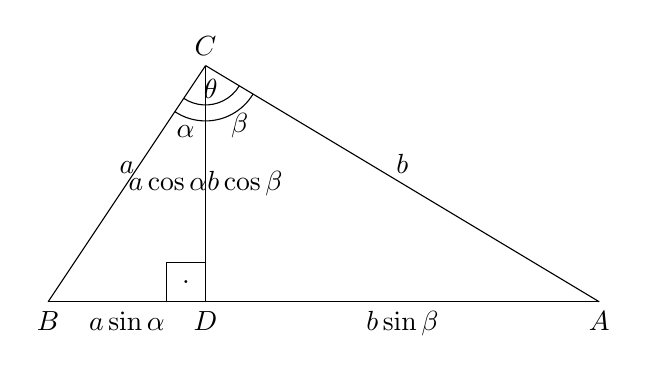
\begin{tikzpicture}
        \coordinate[label=below:$A$] (a) at (7,0); 
        \coordinate[label=below:$B$] (b) at (0,0); 
        \coordinate[label=above:$C$] (c) at (2,3); 
        \coordinate[label=below:$D$] (d) at (2,0); 
        \draw (b) -- (d) node[midway,anchor=north]{$a
        \sin\alpha$};
        \draw (d) -- (a) node[midway,anchor=north]{$b
        \sin \beta$};
        \draw (b) -- (c) node[midway,anchor=south]{$a$};
        \draw (c) -- (a) node[midway,anchor=south]{$b$};
        \draw (c) -- (d) node[midway,anchor=center]{$a \cos \alpha b \cos\beta$};
        \pic[draw, "$\alpha$", angle eccentricity=1.25, angle radius=20] {angle = b--c--d};
        \pic[draw, "$\beta$", angle eccentricity=1.25, angle radius=20] {angle = d--c--a};
        \pic[draw, "$\theta$"] {angle = b--c--a};
        \pic[draw, "$.$", angle eccentricity=.5] {right angle = c--d--b};
        \end{tikzpicture}
    \caption{}
    \label{fig:cos_law_tri}
\end{figure}
Figure~\ref{fig:cos_law_tri} shows a triangle with rules below
\begin{align}
    |BC| &= a \\
    |AC| &= b \\
    |BD| &= a\sin\alpha \\   
    |AD| &= b\sin\beta \\
    |CD| &= a\cos\alpha = b\cos\beta\\
    |AB| &= |BD|+|AD|\\
    |CD| \bot |AB|\\
    \angle{BCD} &= \alpha\\
    \angle{DCA} &= \beta \\
    \angle{BCA} &= \theta = \angle{BCD} + \angle{DCA}
\end{align}


\begin{align}
    c &= a\sin\alpha + b\sin \beta\\
    c^2 &= a^2\sin^2 \alpha + b^2\sin^2 \beta + 2ab\sin\alpha\sin \beta\\
     &= a^2\sin^2 \alpha + b^2\sin^2 \beta + 2ab[\cos \alpha\cos\beta - \cos(\alpha +\beta)]\ \text{by trigonometric identities}\\
     &= a^2\sin^2 \alpha + b^2\sin^2 \beta + ab\cos \alpha\cos\beta + ab\cos \alpha\cos\beta - 2ab\cos(\alpha +\beta)\\
     &= a^2\sin^2 \alpha + b^2\sin^2 \beta + a^2\cos^2 \alpha + b^2\cos^2 \beta - 2ab\cos(\alpha +\beta)\\
     &= a^2(\sin\alpha^2 + \cos \alpha^2) + b^2(\sin^2 \beta + \cos^2 \beta) - 2ab\cos(\alpha +\beta)\\
     &= a^2 + b^2 - 2ab\cos(\alpha +\beta)\\
     &= a^2 + b^2 - 2ab\cos \theta \label{cos_law}
\end{align}
\subsection{Relation Between Dot Product and Cosine} 
Assuming that $a, b$ and $c$ are vectors and
\begin{equation}
    c = a-b
\end{equation} 
With the properties in~\ref{dotp} mind
\begin{align}
    c^2 &= (a-b)^T(a-b)\\
    &= a^Ta +b^Tb - 2a^Tb\\
\end{align}
Using~\ref{cos_law}
\begin{align}
    a^Ta +b^Tb - 2a^Tb &= \norm{a}^2 + \norm{b}^2 - 2\norm{a}\norm{b}\cos \theta\\
    a^Tb &= \norm{a}\norm{b}\cos \theta~\cite{nowell_math_2006}
\end{align}
Now for a given point $p$ and normal vector $a$, every point $x$ making $a$ and $(x-p)$ perpendicular to each other ($\theta = \frac{\pi}{2}$) 
\begin{align}
    a^T(x-p) &= 0\\
    a^Tx-a^Tp &= 0\\
    a^Tx+b &= 0
\end{align}
indeed spans a hyperplane. Notice $b = -a^Tp$ is a constant scalar. We have proven the hyperplane equation as well
\subsection{Jensen's Inequality}
Continuing from our results in previous part, we extract the last feature of $x$ with its corresponding coefficient, to bring an axis of reference to our analysis
\begin{align}
    a^Tx+b &= 0\\
    a_{1:N-1}^Tx+a_Ny+b &= 0 \label{hyperplane_eq}
\end{align}
Then we bring up a hypersurface with 
\begin{equation}
    y=f(x) \label{hypersurf_eq}
\end{equation}
which intersects the plane in a region $\Omega$ such that their intersecting region $\Omega_c$ is the boundary of $\Omega$. $f$ is either convex (i.e. a bowl placed on a table in 3D, $y$ increasing toward the sky) or concave (i.e. the bowl upside down in 3D) within $\Omega$. Within $\Omega_c$, we can take any set of points as column vectors organized as a matrix
$$
X = \begin{bmatrix}
    x_0 & x_1 & ... & x_M
\end{bmatrix}
$$
It is easy to see that $X$ satisfies both~\ref{hyperplane_eq} and~\ref{hypersurf_eq}. Let us multiply both sides with a vector of weights $c$ whose Manhattan norm is 1 (sum of its items adds up to 1). 
\begin{align}
    a_{1:N-1}^TX+(a_Ny+b)1^T &= 0\\
    a_{1:N-1}^TXc+(a_Ny+b)1^Tc &= 0\\
    a_{1:N-1}^TXc+a_Ny+b &= 0
\end{align}
Whenever only one element $c_i=1$ (and trivially others are zero of course), we have
\begin{align}
    a_{1:N-1}^Tx_i+a_Nf(x_i)+b = 0\\
    a_{1:N-1}^Tx_ic_i+a_Nf(x_i)c_i+bc_i = 0\\
    \sum_i a_{1:N-1}^Tx_ic_i+\sum_i a_Nf(x_i)c_i+\sum_i bc_i = 0\\
    a_{1:N-1}^T\sum_i x_ic_i+a_N\sum_i f(x_i)c_i+b = 0\\
\end{align}
We have shown for a point $x_c=Xc$ 
\begin{equation}
    y(Xc)=f(X)c=\sum_i c_if(x_i)
\end{equation}
We will further assume for all $i$, $c_i \in [0,1]$
\begin{align}
    \min_kx_{kj} &\leq x_{ij} \leq \max_kx_{kj}\\
    c_i\min_kx_{kj} &\leq c_ix_{ij} \leq c_i\max_kx_{kj}\\
    \sum_i c_i\min_kx_{kj} &\leq \sum_i c_ix_{ij} \leq \sum_i c_i\max_kx_{kj}\\
    \min_kx_{kj} &\leq \sum_i c_ix_{ij} \leq \max_kx_{kj}\\
\end{align}
We see that $x_c$ lies within a subregion of $\Omega$, hence by definition of convexity of surface, 
\begin{equation}
    f(Xc) = 
    \begin{cases}
        \leq  f(X)c & \text{if $f$ is convex}\\
        \geq  f(X)c & \text{if $f$ is concave}
    \end{cases}
\end{equation}
\subsection{Positive Semi-definiteness of a Matrix of the Form $X^TX$}
Let $A$ be a symmetric square matrix, and also $A=X^TX$. For any vector $z$, 
\begin{equation}
z^TAz = z^TX^TXz = (Xz)^T(Xz) \geq 0
\end{equation}
Since squared norm is non-negative, $A=X^TX$ is positive semi-definite.
\subsection{Existence of a (Trivially Unique) Orthonormal Basis of Eigenvectors for a Symmetric Diagonalizable Matrix}
Let $A$ be a diagonalizable symmetric square matrix. Let $P$ be a square matrix such that it's $i$th column $v_i$ is the $i$th eigenvector of $A$. Let $\Lambda$ be the diagonal matrix whose $i$th diagonal $\lambda_i$ is the eigenvalue corresponding to $v_i$. According to definition of eigenvalues/eigenvectors.
\begin{align}
    AP &= P\Lambda\\
    A &= P\Lambda P^{-1}\\
    \Lambda &= P^{-1}AP\\
    \lambda_iv_i &= Av_i\\
    \lambda_iv_i^T &= v_i^TA^T\\
    \lambda_iv_i^Tv_j &= v_i^TA^Tv_j\\
    &= v_i^TAv_j\\
    &= \lambda_jv_i^Tv_j\\
    (\lambda_i-\lambda_j)v_i^Tv_j &= 0
\end{align}
Since $A$ is diagonalizable, $\lambda_i=\lambda_j$ if and only if $i=j$. Hence if $i \neq j$, $v_i^Tv_j = 0$ and $P$ is orthogonal~\cite{magidin_linear_2011}, hence 
$PP^T = D$ such that 
\begin{equation}
D_{ij} = \begin{cases}
    |v_i|^2 & i = j\\
    0 & \text{otherwise}
\end{cases}
\end{equation}
We can have $P' = PD^{-\frac{1}{2}}$, and $\Lambda' = \Lambda D = D^{\frac{1}{2}} \Lambda D^{\frac{1}{2}}$. Then
\begin{equation}
    A = P'\Lambda'P'^T 
\end{equation}
such that $P'$ is orthonormal. We are going to reference $P'$ and $\Lambda'$ as $P$ and $\Lambda$ respectively. We have shown that any symmetric diagonalizable matrix has orthonormal basis of eigenvectors.
\subsection{Relation Between Definiteness and Sign of the Eigenvectors}
\begin{align}
    z^TAz &= z^TP\Lambda P^Tz\\
    &= (P^Tz)^T\Lambda (P^Tz)\\
    &= \sum_i (P^Tz)_i^2 \lambda_i\\
    &= \sum_i z'_i^2 \lambda_i
\end{align}
The term is actually sum of eigenvalues weighted by values of $z'$, which has the same norm as $z$ due to the fact that $P$ is orthonormal. For all $z$ (hence $z'$), the weighted sum is non-negative if and only if $A$ is semi-positive definite. Non-negativity in this case is guaranteed when all eigenvectors are non-negative. This approach also works for other types of definite matrices (we cannot say anything about indefinite matrices). 
\subsection{Relation Between Invertability and Definiteness}
For any diagonalizable matrix $A$, 
\begin{align}
    det(A) &= det(P) det(\Lambda) det(P^{-1})\\
    &= det(P) det(\Lambda) \frac{1}{det(P)}\\
    &= det(\Lambda)\\
    &= \prod_i \lambda_i
\end{align}
We see that the semi-definite matrices are not invertible since they have at least one zero eigenvalue. We have shown that semi-definite matrices are not invertible and definite matrices are invertible.
\subsection{Definiteness of Hessian Matrix to Determine Curvature Near Critical Points}
\subsubsection{Quadratic Function}
Let $q(x)$ be a quadratic function with $\prescript{d \times d}{}{A}, \prescript{d \times 1}{}{x}, \prescript{d \times 1}{}{b}$ and a scalar $c$
\begin{equation}
    q(x) = x^TAx+x^Tb+c
\end{equation}
of the form where $A$ is symmetric.
\begin{align}
    \nabla q(x) &= (A+A^T)x+b\\
     &= 2Ax+b
\end{align}
The critical point $x^* = -\frac{1}{2}A^{-1}b$ where $\nabla q(x^*) = 0$.
\begin{align}
    q(x^*+\Delta x) &= q(x^*) + \Delta x^TA\Delta x + 2\Delta x^TAx^* + \Delta x^Tb\\
    &= q(x^*) + \Delta x^TA\Delta x
\end{align}
We can deduce from previous results, 
\begin{itemize}
    \item $\forall \Delta x [q(x^*) < q(x^*+\Delta x)]$ if $A$ is positive definite ($x^*$ is minimum, minimization problem)
    \item $\forall \Delta x [q(x^*) > q(x^*+\Delta x)]$ if $A$ is negative definite ($x^*$ is maximum, maximization problem)
    \label{posneg}
\end{itemize}
If $A$ is indefinite, then depending on $\Delta x$, $q(x^*)$ can be less or greater than $q(x^*+\Delta x)$, which means $x^*$ is a saddle point. Since semi-definite matrices are not invertible we cannot use $x^* = -\frac{1}{2}A^{-1}b$. If $A$ is semi-definite, for some $x$, we have $q(x) = x^Tb+c$ (a hyperplane with a $d+1$-dimensional normal having scalars of $b$ and having $1$ in the dimension of a reference axis, i.e. inclined-plane). If $b$ is zero, then we have infinitely many critical points (a hyperplane with a normal along the reference axis, i.e. ground-plane).

Let $d$ be an arbitrary vector.
\begin{align}
    \nabla q(x^* + Pd) &= 2A(Pd + x^*)+b\\
    &= 2(P\Lambda P^T)(Pd + x^*)+b\\
    &= 2P\Lambda P^TPd + 2Ax^*+b\\
    &= 2P\Lambda d\\
    &= \sum_i 2d_i\lambda_i v_i\\
    \nabla q(x^*+Pd)^T \nabla q(x^*+Pd) &= (2P\Lambda d)^T2P\Lambda d\\
    &= 4d^T\Lambda P^TP\Lambda d\\
    &= 4d^T\Lambda^2 d\\
    &= \sum_i 4d_i^2  \lambda_i^2\\
    &= \bar{c}^2 \quad \text{For an arbitary scalar $\bar{c}$}\\
    \sum_i \frac{d_i^2}{\frac{\bar{c}^2}{4\lambda_i^2}} &= 1
\end{align}
We have shown that contours (curves where gradient magnitudes/norms are equal) are ellipsoids.
\begin{equation}
    \nabla q(x^* + \frac{\bar{c}}{2\lambda_i}v_i) = \bar{c}v_i
\end{equation}
in a contour with multiplier $\bar{c}$. The eigenvector $v_i$ is a unit direction along a principal semi-axis of the ellipsoid. Note that in order to reach to a contour with multiplier $\bar{c}$ from $x^*$, the magnitude/norm of the vector is $\frac{\bar{c}}{2\lambda_i}$. As $\lambda_i$ increases, the magnitude/norm decreases, and vice-versa.

For any function, $f(x)$ its second order Tailor expansion approximates it in the neighbor of $x$.
\begin{equation}
    f(x+\Delta x) \approx f(x)+\Delta x^T\nabla f(x)+\Delta x^TH(x)\Delta x
\end{equation}
where $H(x) = \nabla^2f(x)$ is Hessian of $f(x)$. Substituting $A$, $b$ and $c$, this approximation can be used to determine the behavior of $f$ near $x$ in optimization algorithms such as gradient descent (where $\Delta x$ is learning rate times the gradient). For example if $H(x)$ is semi-definite, this time we have a plateau, as plateau is a plane near $x$ (ground or inclined).

\subsubsection{Arbitrary Gaussian Function}
Let $g(x) = he^{q(x)}$, with an arbitrary scalar $f$. 
\begin{equation}
    \nabla g(x) = \nabla q(x) g(x)
\end{equation}
We see that the critical points of $g(x)$ are the same as of $q(x)$. 
\begin{align}
    g(x^*+\Delta x) &= he^{q(x^*+\Delta x)}\\
     &= he^{q(x^*) + \Delta x^TA\Delta x}\\
     &= e^{\Delta x^TA\Delta x}g(x^*)
\end{align}
Similarly deductions from part~\ref{posneg} can be made. Same as that part, If $A$ is indefinite, then depending on $\Delta x$, $g(x^*)$ can be less or greater (saddle point). If $A$ is semi-sefinite, for some infinitely many $x$, we have $g(x) = e^{x^Tb+c}$ (inclined-plane). If $b$ is zero, then we have infinitely many critical points (ground-plane). Otherwise, we have no critical points at all.
\begin{align}
    \nabla g(x^*+Pd) &= \nabla q(x^*+Pd) g(x^*+Pd)\\
    &= (2P\Lambda d) e^{(Pd)^TA(Pd)}g(x^*)\\
    &= (2P\Lambda d) e^{d^TP^TAPd}g(x^*)\\
    &= (2P\Lambda d) e^{d^T\Lambda d}g(x^*)\\
    \nabla g(x^*+Pd)^T \nabla g(x^*+Pd) &= (\sum_i 4d_i^2\lambda_i^2)e^{2d^T\Lambda d}g(x^*)^2\\
    &= (\sum_i 4d_i^2\lambda_i^2)e^{\sum_i 2d_i^2\lambda_i}g(x^*)^2\\
    (\sum_i 4d_i^2\lambda_i^2)e^{\sum_i 2d_i^2\lambda_i}g(x^*)^2 &= \bar{c}^2
\end{align}
Note that after this point, I could not come with a rigorous proof, but used a computer.
If we use density function of normal distribution which is a special case of $g(x)$ with $b=-2A\mu$ ($x^*$ becomes $\mu$), $c=\mu^TA\mu$, $f = \frac{1}{\sqrt{(2\pi)^n}det(A)} = \frac{1}{\sqrt{(2\pi)^n\prod_j \lambda_j}}$ (to have infinite integral equal 1 by definition of density functions), and inputting the values to a calculator (I used Desmos), the function behaves like an ellipsoid having eigenvectors along its principal semi-axes. please note that $A=-\frac{1}{2}\Sigma^{-1}$, where covariance matrix $\Sigma$ needs to be positive definite (it can trivially be semi-positive definite in the limit for generalization). Therefore, $A$ is negative definite, having all negative eigenvalues. As I increased the eigenvalues, the length of the principal semi-axis corresponding to the eigenvector has decreased. 
This analysis gives ellipsidicity information of the Gaussian that is fitted to a normally distributed sample. 
\section{Probability Theory and Statistics Concepts Used In Learning}
\subsection{Distinction Between Correlation and Dependence}
\label{cor_dep}
We have seen the relationship between eigenvectors/values and the covariance matrix. Assume that we fitted a continuous normal distribution to an elliptic
sample of data in order to estimate the most probable regions of occurence, the properties of the continuous distribution will also approximate the properties of the sample. If we squish the sample more, the data will be better approximated with a more squished Gaussian. Remember from the previous parts along the axis of compression, the eigenvalue corresponding to that axis will become larger. At some point it will be the largest eigenvalue and the data will be approximated by a hyperplane with the normal being its eigenvector (1D hyperplane is a line). We say, such data has a \textit{linear dependence}. However, dependence -relation between axes/dimensions/features in the data- is a more general concept and the covariance matrix only gives information about linear dependence. There can be infinitely many other types such as quadratic, cubic and so on. Correlation is a subset of dependence. When a number of random variables are independent of each other (i.e. mutual independence), they don't have any dependence whatsoever; hence they also become uncorrelated, but the reverse condition does not hold. In other words, independence implies uncorrelatedness but not vice-versa
\subsection{Probabilistic Chain Rule Equations With Independent Random Variables}
\subsubsection{Conditional Mutual Independence}
\label{cond_mutual_independence}
Assume there exists an array of hidden and observed variables $X$ and $Y$ respectively. For example in a classification task, $X$ can be the raw pixel values of an image whereas $Y$ is whether the image is a cat or not. In a regression task, $X$ can be a tabular data row of a house whereas $Y$ is the price. $X$ is sampled from a prior $p(x)$.

Further assume, for $i \neq j$, $y_i, y_j$ are conditionally independent given $x$ (1), and $x_i, y_i$ are conditionally independent given $x_j$ (2). You can think of the vector as the data and pairs $(x,y)$ as points such that the point $y_i$ is label of $x_i$. Using~\ref{cond_independence1} and~\ref{cond_independence2}
\begin{align}
    p(y|x) &= \prod_i p(y_i|x)\\
           &= \prod_i p(y_i|x_i)
\end{align}
If we use natural language, then we can say (as also proven above) $y_i$ depends only on $x_i$. This is the foundational assumption that people build their learning models on. Note that $x_i$ can be further divided into features $x_{ij}$ that could be correlated among each other. Then we can further remove those features in the equation above, still having the same result $p(y|x)$. 

People use dimension reduction algorithms such as PCA to find those correlated features for removal. PCA simply finds the line having eigenvector with the largest eigenvalue as its normal. Than merges the features affected by this eigenvector. One may iteratively drop the features until the desired dimension.
\subsubsection{Markov Property and Markov Chain}
Markov property is defined for a stochastic process when the future only depends on the present. Using the equation~\ref{cond_independence1} along this definition gives
\begin{equation}
    p(x_t|x_{t-1},x_{t-2},...,x_0) = p(x_t|x_{t-1})
\end{equation}
Using the equation~\ref{joint_cond_prob}, we can recursively expand any joint probability as follows
\begin{align}
    p(x_{0:T}) &= p(x_0,x_1,...,x_T) \\
    &= p(x_0)\prod_{t=1}^T p(x_t|x_{t-1},x_{t-2},...,x_0)\\
    p(x_{1:T}|x_0) &= \prod_{t=1}^T p(x_t|x_{t-1},x_{t-2},...,x_0)
\end{align}
If we further assume the process involving $p$ has markov property, then
\begin{align}
    p(x_{0:T}) &= p(x_0)\prod_{t=1}^T p(x_t|x_{t-1}) \label{markov_chain_joint}\\
    p(x_{1:T}|x_0) &= \prod_{t=1}^T p(x_t|x_{t-1}) \label{markov_chain_cond}
\end{align}
\subsection{Non-negativity of KL-Divergence}
\label{kl_nonneg}
Negative of any function switches its convexity property (i.e. reversing the bowl on the table). Using the definition of KL-Divergence, the Jensen's inequality and the fact that logarithm is a concave function 
\begin{align}
     \int_X p(X)\log\frac{p(X)}{q(X)} dX &= \int_X p(X)(-\log)\frac{q(X)}{p(X)} dX\\
     &\geq -\log \int_X p(X)\frac{q(X)}{p(X)} dX\\
     &\geq -\log \int_X q(X) dX\\
     &\geq -\log \int_X q(X) dX\\
     &\geq -\log 1 \\
     &\geq 0
\end{align}
Bear in mind that this was true because our assumptions of having a vector of all positive entries and Manhattan norm of 1 aligns with the probability distribution (Integral is a type of sum).
\subsection{Monotonicity of KL-Divergence}
A function $f$ is \textit{monotonically decreasing} if
\begin{equation}
    f(x) \leq f(y) \longleftrightarrow x \geq y
\end{equation}
similarly, there is also increasing monotonicity which is irrelevant at this point. We will show for any probability distributions $p(x)$ and $q(x)$, $KL(p(x)\parallel q(x))$ is monotonically decreasing in every direction. We can take derivatives and look at the behavior of the function for that. For simplicity, we use continuous indexing such that $p(x_i)=p_i$ 
\begin{align}
    \frac{\delta}{\delta q_j}\int_i p_i\log\frac{p_i}{q_i} di &= \int_i p_i\frac{\delta}{\delta q_j}\log\frac{p_i}{q_i} di\\
    &= p_j\frac{-\frac{p_j}{q_j^2}}{\frac{p_j}{q_j}}\\
    &= -\frac{p_j}{q_j} \label{klmonotonicity}
\end{align}
Let us keep $p$ constant for now and express KL-divergence as a function of $q$ (i.e. $KL(q)$). Because $p$ has to sum up to 1, in at least one dimension $k$,~\ref{klmonotonicity} is always negative (but not zero), so KL-divergence is strictly decreasing in that dimension. Then KL-divergence is strictly decreasing in every dimension. In this regard having two points $q_1$ and $q_2$, $KL(q_1)=KL(q_2)$ if and only if $q_1=q_2$, hence the only $q$ that will reach the minimum of zero is $q=p$.
\subsection{Cross-Entropy}
\subsubsection{General Derivation}
\label{ce_derivation}
In ML problems, we want to find the underlying distribution $q(y|x)$. Looking at the ~\ref{bayesian}, we can find the posterior if the likelihood and the prior are \textit{tractable} (their closed form can be found), which is not generally the case. Therefore, people tend to learn another distribution $p(y|x,\theta)$ with parameters $\theta$. The ideal distribution $p(y|x,\theta)$ should be equal to $q(y|x)$, which is equivalent to saying that the difference $KL(q(y|x)\parallel p(y|x,\theta))$ should be zero. Then the optimum parameters
\begin{align}
    \hat{\theta} 
    &= \arg_\theta \min[KL(q(y|x) \parallel p(y|x,\theta))]\\
    &= \arg_\theta \min[ KL(q(y|x) \parallel p(y|x,\theta)) + H(q(y|x))]\\
    &= \arg_\theta \min \left( E_{q(y|x)}\Big[\log\frac{q(y|x)}{p(y|x,\theta)}\Big] + E_{q(y|x)}\Big[-\log q(y|x)\Big]\right)\\
    &= \arg_\theta \min \left( E_{q(y|x)}\Big[-\log p(y|x,\theta)\Big]\right)\label{ce_derivation_res}\\
    &= \arg_\theta \min H(q(y|x), p(y|x,\theta))
\end{align}
\subsubsection{Relationship With Maximum Likelihood Estimator (MLE) for Supervised Tasks}
\label{mle_ce}
Continuing from~\ref{ce_derivation_res}, 
\begin{equation}
    = \arg_\theta \min \sum_j -q(y=j|x)\log p(y=j|x,\theta)
\end{equation}
We will assume $q$ is known (see~\ref{catdist}).
\begin{align}
    &= \arg_\theta \min \sum_j -(1\{y=j\})\log p(y=j|x,\theta)\\
    &= \arg_\theta \min \sum_j -\log p(y=j|x,\theta)^{1\{y=j\}}\\
    &= \arg_\theta \max \sum_j \log p(y=j|x,\theta)^{1\{y=j\}}\\
    &= \arg_\theta \max\left[\log\prod_j p(y=j|x,\theta)^{1\{y=j\}}\right]\\
    &= \arg_\theta \max\left[\exp\Big(\log\prod_j p(y=j|x,\theta)^{1\{y=j\}}\Big)\right]\\
    &= \arg_\theta \max\prod_j p(y=j|x,\theta)^{1\{y=j\}}\\
    &= \arg_\theta\max p(y|x,\theta) \ \text{(see~\ref{catdist})}\\
    &= \hat{\theta}_{MLE}\label{mle_ce_res}
\end{align}
We conclude that minimizing the corresponding loss is equivalent to finding the maximum likelihood of the output $Y$ wrt the input $X$ and the parameters $\theta$. 
\subsection{Mean Squared Error}
\subsubsection{General Derivation}
\label{mse_derivation}
We assume $p(y|x,\theta) = \mathcal{N}(y; \mu_\theta(x),\sigma^2)$ and $q(y|x) = \mathcal{N}(y; \mu(x),\beta)$. We will obtain the result using KL-divergence. Deriving the equation below, Gupta made our life easier.
\begin{equation}
    p(x) = \mathcal{N}(x;\mu_p,\Sigma_p), q(x) = \mathcal{N}(x;\mu_q,\Sigma_q) \longleftrightarrow KL(p(x) \parallel q(x)) = \frac{1}{2}\left[(\mu_p-\mu_q)^T\Sigma_q^{-1}(\mu_p-\mu_q) + tr\left\{\Sigma_q^{-1}\Sigma_p\right\}+\log\frac{|\Sigma_q|}{|\Sigma_p|} - k\right]~\cite{gupta_kl_2020}\label{gupta_kl}
\end{equation}
Vectors $x_i, y_i, \mu_i=\mu(x_i)$ and $\mu_\theta(x_i)$ share the same number $k$ of dimensions/features. Substituting gives
\begin{align}
    \hat{\theta} 
    &= \arg_\theta \min[KL(q(y|x) \parallel p(y|x,\theta))]\\
    &= \arg_\theta \min\frac{1}{2}\left[\frac{1}{\sigma^2}\big(\mu-\mu_\theta(x)\big)^2 + \frac{\beta}{\sigma^2}+k\log\frac{\sigma^2}{\beta} - k\right]\\
    &= \arg_\theta \min\frac{1}{2\sigma^2}\big(\mu-\mu_\theta(x)\big)^2\label{mse_derivation_res2}
\end{align}

People may experiment with different constants $\frac{1}{2\sigma^2}$ and see whichever is the top performing as long as~\ref{minmaxcomp1} and~\ref{minmaxcomp2} are satisfied (it does for all due to the square as variance cannot be negative).
\subsubsection{Relationship With Maximum Likelihood Estimator (MLE) for Supervised Tasks}
\label{mle_mse}
Continuing from~\ref{mle_ce_res} with the assumption $p(y|x,\theta) = \mathcal{N}(y; \mu_\theta(x),\sigma^2)$; hence, 
\begin{align}
    \hat{\theta}_{MLE} 
    &= \arg_\theta \max p(y|x,\theta)\\
    &= \arg_\theta \max \frac{1}{(\sigma\sqrt{2\pi})^k}\exp\Big(-\frac{1}{2\sigma^2}(\mu_\theta(x)-y)^2\Big)\\
    -\log\hat{\theta}_{MLE} &= \arg_\theta\min\left[-\log\left(\frac{1}{(\sigma\sqrt{2\pi})^k}\exp\Big(-\frac{1}{2\sigma^2}(\mu_\theta(x)-y)^2\Big)\right)\right]\\
    &= \arg_\theta\min[-k\log(\sigma\sqrt{2\pi}) + \frac{1}{2\sigma^2}(\mu_\theta(x)-y)^2]\\
    &= \arg_\theta \min\frac{1}{2}(\mu_\theta(x)-y)^2\ \text{after eliminating the constants}
    \label{mse_derivation_res1}
\end{align}
Remember that we have a freedom when removing the constants as long as they comply with ~\ref{minmaxcomp1} and~\ref{minmaxcomp2}. In this regard, we did not eliminate $\frac{1}{2}$ for convenience, as taking derivatives will remove it anyways. 

Notice that in~\ref{mle_ce}, we are approximating a probability distribution (minimizing KL-divergence) between $\hat{y} = p(y|x,\theta)$ and an underlying distribution $q(y|x)$ with labels $y$ (whose hot-encoding is the distribution itself). However, when substituting with the Gaussian, we see we are fitting a Gaussian by minimizing the distance of its mean to the datapoint $y$.  
\subsection{Loss Function as a Sum of Elements in Supervised Tasks}
For supervised tasks, we found a relationship between MLE and the loss functions $\mathcal{L}_\theta(\hat{y},y)$ in~\ref{mle_ce} and~\ref{mle_mse} for a single data point $(x,y)$. What about a dataset? We start with an assumption again that the variables $X$ and $Y$ are independent as given in~\ref{cond_mutual_independence}. Then 
\begin{align}
    \hat{\theta}_{MLE} 
    &= \arg_\theta \max p_{model}(y|x,\theta)\\
    &= \arg_\theta \max \prod_i p_{model}(y_i|x_i,\theta)\\
    -\log\hat{\theta}_{MLE}
    &= \arg_\theta \min \sum_i -\log p_{model}(y_i|x_i,\theta)\\
    &= \arg_\theta \min \sum_i \mathcal{L}_\theta(\hat{y_i},y_i)\label{loss_sum_res}
\end{align}
If we multiply multiple single variable Gaussians, we reach the formula, in~\ref{normal_specific}, having a diagonal covariance matrix. In this case, the features are uncorrelated ($Cov(x_i,x_j)=0$ if $i \neq j$), hence mutually independent, not contradicting our claim in~\ref{cor_dep}. In this case, we are also claiming $p(y|x,\theta)=\mathcal{N}(y; \mu_\theta(x),\sigma^2)$.
\subsection{Expected Value of Multiple Variables}
\label{multi_mean_derivation}
Here, we are proving that the expected value has the superposition property
\begin{align}
     E_{p(X,Y)}[X] 
     &= \int_X\int_Y p(X,Y)X dX dY = E_{X,Y}[X]\\
     &= \int_X\Big(\int_Y p(X,Y)dY\Big) X dY = E_{X}[E_{Y}[X]] = E_{X}[E_{Y}[1]X]\\
     &= \int_X p(X) X dX = E[X]\\
     E_{p(X,Y)}[X] 
     &= \int_X\int_Y p(X,Y)X dX dY\\
     &= \int_X\Big(\int_Y p(X,Y)dY\Big) X dY\\
     &= \int_X p(X) X dX\\
     &= E[X]\\
    E[aX+bY] 
    &= E_{p(X,Y)}[aX+bY]\\
    &= aE_{p(X,Y)}[X]+bE_{p(X,Y)}[Y]\ \text{due to linearity of the integral}\\
    &= aE_{p(X)}[X]+bE_{p(Y)}[Y]\\
    &= aE[X]+bE[Y]
\end{align}
recursively expanding, it is easy to see this equation applies to the general case
\begin{align}
    E\big[\sum_{i=1}^N a_iX_i\big] &= a_1E[X_1]+E\big[\sum_{i=2}^N a_iX_i\big]\\
    &= a_1E[X_1]+a_2E[X_2]+E\big[\sum_{i=3}^N a_iX_i\big]\\
    & ...\\
    &= \sum_{i=1}^N a_iE[X_i]~\label{mean_superpos}
\end{align}
\subsection{Covariance of Multiple Variables}
Here, we are deriving an equation similar to part~\ref{multi_mean_derivation}
\begin{align}
    Cov(aX+bY,cZ+dT) 
    &= E[(aX+bY-\mu_{aX+bY})(cZ+dT-\mu_{cZ+dT})]\\
    &= E[(a(X-\mu_X)+b(Y-\mu_Y))(c(Z-\mu_Z)+d(T-\mu_T))]\\
    &= E[ac(X-\mu_X)(Z-\mu_Z)+ad(X-\mu_X)(T-\mu_T)+bc(Y-\mu_Y)(Z-\mu_Z)+bd(Y-\mu_Y)(T-\mu_T)]\\
    &= acE[(X-\mu_X)(Z-\mu_Z)]+adE[(X-\mu_X)(T-\mu_T)]+bcE[(Y-\mu_Y)(Z-\mu_Z)]+bdE[(Y-\mu_Y)(T-\mu_T)]\\
    &=acCov(X,Z)+adCov(X,T)+bcCov(Y,Z)+bdCov(Y,T)\label{cov_derivation_res}
\end{align}
We will use mathematical induction to prove the general case. assuming the equation
\begin{equation}
    Cov(\sum_{i=1}^{m-1} a_i X_i, \sum_{i=1}^{n-1} b_i Y_i) = \sum_{i=1}^{m-1} \sum_{j=1}^{n-1} a_i b_j Cov(X_i, Y_j)
\end{equation}
holds, it is trivial to see for 
\begin{equation}
    Cov(\sum_{i=1}^{m} a_i X_i, \sum_{i=1}^{n} b_i Y_i) = Cov(\sum_{i=1}^{m-1} a_i X_i + a_m X_m, \sum_{i=1}^{n-1} b_i Y_i + b_n Y_n)
\end{equation}
\begin{equation}
    \begin{split}
        =Cov(\sum_{i=1}^{m-1} a_i X_i,\sum_{i=1}^{n-1} b_i Y_i)+\underbrace{b_nCov(\sum_{i=1}^{m-1} a_i X_i,Y_n)}_{c_1}+
        \underbrace{a_mCov(X_m,\sum_{i=1}^{n-1} b_i Y_i)}_{c_2}+a_m b_nCov(X_m,Y_n)
    \end{split}
\end{equation}
For $c_1$ and $c_2$, substituting the coefficients in~\ref{cov_derivation_res}, we can recursively expand the sum until its components as below.
\begin{equation}
    \begin{split}
         =\sum_{i=1}^{m-1} \sum_{j=1}^{n-1} a_i b_j Cov(X_i, Y_j)+\underbrace{b_n\sum_{i=1}^{m-1} a_iCov(X_i, Y_n)}_{c_1}+\underbrace{a_m\sum_{j=1}^{n-1} b_j Cov(X_m, Y_j)}_{c_2}+a_m b_nCov(X_m,Y_n)
    \end{split}
\end{equation}
\begin{equation}
    \begin{split}
         =\sum_{i=1}^{m} \sum_{j=1}^{n} a_i b_j Cov(X_i, Y_j)
    \end{split}
\end{equation}
concluding the proof.
\subsection{Variance of Multiple Variables}
Using the fact that variance is just the \textit{self-covariance}
\begin{align}
    Var(\sum_{i=1}^{n} a_i X_i) &= Cov(\sum_{i=1}^{n} a_i X_i, \sum_{i=1}^{n} a_i X_i)\\
    &= \sum_{i=1}^{n} \sum_{j=1}^{n} a_i a_j Cov(X_i, X_j)\\
    &= \sum_{i=1}^{n} a_i^2 Cov(X_i, X_i) + \sum_{i=1}^{n} \sum_{j \neq i}^{n} a_i a_j Cov(X_i, X_j)\\
    &= \sum_{i=1}^{n} a_i^2 Var(X_i) + \sum_{i=1}^{n} \sum_{j \neq i}^{n} a_i a_j Cov(X_i, X_j)\\
    &= \sum_{i=1}^{n} a_i^2 Var(X_i)\ \text{(assuming $X$ is uncorrelated)}\label{var_derivation_res}\\
\end{align}
\subsection{Preference of Mean over Summation for Loss Functions in Supervised Tasks}
\label{mean_loss}
Deriving~\ref{loss_sum_res} for a dataset, we see a pattern in which we try to minimize a sum.
Using~\ref{var_derivation_res}, for a sample $X_{1:n}$ with constant variance $\sigma^2$, the variance of the sample mean,
\begin{align}
    Var(\overline{X}) &= Var(\frac{1}{n}\sum_{i=1}^{n} X_i)\\
    &= \frac{1}{n^2} \sum_{i=1}^{n} Var(X_i)\\
    &= \frac{1}{n^2} \sum_{i=1}^{n} \sigma^2\\
    &= \frac{1}{n^2} n \sigma^2\\
    &= \frac{\sigma^2}{n}\\
    Std(\overline{X}) &= \sqrt{Var(\overline{X})}\\
    &= \frac{\sigma}{\sqrt{n}}
\end{align}
We realize that as number of samples increases, the mean of the sample approximates the true mean of the distribution better. That is why people usually use mean instead of sum. Hence new expression for the loss function becomes 
\begin{equation}
    \hat{\theta}_{MLE} = \frac{1}{n}\arg_\theta \min \sum_{i=1}^n \mathcal{L}_\theta(\hat{y_i},y_i)
\end{equation}
As $n$ is a constant relative to the parameters, we are still maximizing the likelihood.
\subsection{Overfitting and Bias-Variance Tradeoff}

Assume the variable input, label pairs ($X$,$Y$) in~\ref{cond_mutual_independence} is sampled from a dataset $D$. We model the machine learning algorithm as a mapping $f$ that approximates a system $F(x)=y$. Due to an inherent noise in $F$, $F$ may output different labels $y$ for a given $x$. Then, \textit{expected label} given $x$ is
\begin{equation}
    \bar{y}(x) = E_{y \vert x} \left[Y\right] = \int\limits_y y \, p(y \vert x) dy.
\end{equation}
for all label values $y$ possible.

For each dataset $D$, the optimal mapping $f_D$ predicts $f_D(x) = y^*$. \textit{Expected prediction} given $x$ is
\begin{equation}
    \bar{f}(x) = E_D \left[ f_D(x) \right] = \int\limits_D f_D(x) p(D) dD
\end{equation}
for all datasets $D$ possible. Remember from~\ref{mse_derivation}, if we assume the necessary conditions, we can model the loss as an MSE 
\begin{align}
    \mathcal{L}_D(x,y) &= E_{x,y,D}\left[\left[f_D(x) - y\right]^{2}\right]\\ 
    &= E_{x,y,D}\left[\left[\left(f_D(x) - \bar{f}(x)\right) + \left(\bar{f}(x) - y\right)\right]^{2}\right] \\
    &= E_{x, D}\left[(\bar{f}_{D}(x) - \bar{f}(x))^{2}\right] + E_{x, y} \left[\left(\bar{f}(x) - y\right)^{2}\right] + 2 E_{x, y, D} \left[\left(f_D(x) - \bar{f}(x)\right)\left(\bar{f}(x) - y\right)\right]
\end{align}
\begin{align}
	E_{x, y, D} \left[\left(f_D(x) - \bar{f}(x)\right) \left(\bar{f}(x) - y\right)\right] &= E_{x, y} \left[E_{D} \left[ f_D(x) - \bar{f}(x)\right] \left(\bar{f}(x) - y\right) \right] \\
    &= E_{x, y} \left[ \left( E_{D} \left[ f_D(x) \right] - \bar{f}(x) \right) \left(\bar{f}(x) - y \right)\right] \\
    &= E_{x, y} \left[ \left(\bar{f}(x) - \bar{f}(x) \right) \left(\bar{f}(x) - y \right)\right] \\
    &= E_{x, y} \left[ 0 \right] \\
    &= 0
\end{align}
\begin{equation}
	E_{x, y, D} \left[ \left( f_D(x) - y \right)^{2} \right] = \underbrace{E_{x, D} \left[ \left(f_D(x) - \bar{f}(x) \right)^{2} \right]}_{\text{Variance }(\sigma^2)} + E_{x, y}\left[ \left( \bar{f}(x) - y \right)^{2} \right]
\end{equation}
\begin{align}
	E_{x, y} \left[ \left(\bar{f}(x) - y \right)^{2}\right] &= E_{x, y} \left[ \left(\bar{f}(x) -\bar y(x) )+(\bar y(x) - y \right)^{2}\right]  \\
  &=\underbrace{E_{x, y} \left[\left(\bar{y}(x) - y\right)^{2}\right]}_{\text{Noise }(\epsilon)} + \underbrace{E_{x} \left[\left(\bar{f}(x) - \bar{y}(x)\right)^{2}\right]}_\mathrm{Bias^2} + 2 E_{x, y} \left[ \left(\bar{f}(x) - \bar{y}(x)\right)\left(\bar{y}(x) - y\right)\right]
\end{align}
\begin{align}
	E_{x, y} \left[\left(\bar{f}(x) - \bar{y}(x)\right)\left(\bar{y}(x) - y\right)\right] &= E_{x}\left[E_{y \mid x} \left[\bar{y}(x) - y \right] \left(\bar{f}(x) - \bar{y}(x) \right) \right] \\
    &= E_{x} \left[ E_{y \mid x} \left[ \bar{y}(x) - y\right] \left(\bar{f}(x) - \bar{y}(x)\right)\right] \\
    &= E_{x} \left[ \left( \bar{y}(x) - E_{y \mid x} \left [ y \right]\right) \left(\bar{f}(x) - \bar{y}(x)\right)\right] \\
    &= E_{x} \left[ \left( \bar{y}(x) - \bar{y}(x) \right) \left(\bar{f}(x) - \bar{y}(x)\right)\right] \\
    &= E_{x} \left[ 0 \right] \\
    &= 0
\end{align}
\begin{equation}
	\underbrace{E_{x, y, D} \left[\left(f_D(x) - y\right)^{2}\right]}_{\text{Expected Test Error }(\mathcal{L})} = \underbrace{E_{x, D}\left[\left(f_D(x) - \bar{f}(x)\right)^{2}\right]}_{\text{Variance }(\sigma^2)} + \underbrace{E_{x}\left[\left(\bar{f}(x) - \bar{y}(x)\right)^{2}\right]}_\mathrm{Bias^2} + \underbrace{E_{x, y}\left[\left(\bar{y}(x) - y\right)^{2}\right]}_{\text{Noise }(\epsilon)}~\cite{cornell_2017} 
\end{equation}
Variance $\sigma^2$ here is wrt the datasets $D$. High variance means that the predictions vary a lot by different datasets and vice-versa. 

The bias is simply the squared difference between the predicted and true labels. We use expected labels here since the system (as in a real system) has noise, which is the variance term $\epsilon$ shown above. The noise is generally due to the measurement tools, which we have no impact on. However, we can change the other terms, using methods such as regularization.
\section{Gradients of Functions in Backpropagation}
\subsection{FC (Fully Connected) Layers}
An FC layer implements the function on a set of matrices
\begin{equation}
    \prescript{N\times M}{}{Y} = \prescript{N\times D}{}{X}\prescript{D\times M}{}{W} + \prescript{N\times1}{}{1}\prescript{1\times M}{}{b}
\end{equation}
Using the definition of matrix multiplication in~\ref{matmult}, we have
\begin{equation}
y_{nm} = \sum_{d=1}^D x_{nd} w_{dm}+b_m
\end{equation}
Looking at this definition, we can find partial derivatives 
\begin{align}
    \frac{\delta y_{nm}}{\delta x_{ij}} &= \begin{cases}
        w_{jm} & if\ n=i\\
        0 & \text{otherwise}
    \end{cases}\\
    \frac{\delta y_{nm}}{\delta w_{ij}} &= \begin{cases}
        x_{ni} & if\ m=j\\
        0 & \text{otherwise}
    \end{cases}\\
    \frac{\delta y_{nm}}{\delta b_{j}} &= \begin{cases}
        1 & if\ m=j\\
        0 & \text{otherwise}
    \end{cases}
\end{align}
Using the chain rule with a loss function gives
\begin{align}
    L_{x_{ij}} &= \sum_{n=1}^N\sum_{m=1}^M L_{y_{nm}} \frac{\delta y_{nm}}{\delta x_{ij}}\\
    &= \sum_{m=1}^M L_{y_{nm}} w_{jm}\\
    \prescript{N\times D}{}{L_X} &= \prescript{N\times M}{}{L_Y}\prescript{M\times D}{}{W^T}\\
    L_{w_{ij}} &= \sum_{n=1}^N\sum_{m=1}^M L_{y_{nm}} \frac{\delta y_{nm}}{\delta w_{ij}}\\
    &= \sum_{n=1}^N L_{y_{nm}} x_{ni}\\
    \prescript{D\times M}{}{L_W} &= \prescript{D\times N}{}{X_T}\prescript{N\times M}{}{L_Y}\\
    L_{b_{j}} &= \sum_{n=1}^N\sum_{m=1}^M L_{y_{nm}} \frac{\delta y_{nm}}{\delta b_{j}}\\
    &= \sum_{n=1}^N L_{y_{nm}}\\
    \prescript{1\times M}{}{L_b} &= \prescript{1\times N}{}{1}\prescript{N\times M}{}{L_Y}
\end{align}
\section{Generative Models}
\subsection{Variational Autoencoder}
Autoencoders (AE) are trained with the constraint that input approximates output as closely as possible ($X=Y$). We can model AEs using probabilities similarly to~\ref{cond_mutual_independence} that, we are maximizing the evidence
\begin{align}
    \hat{\theta}_{MLE} &= \arg_\theta\max p_\theta(x)\\ 
    &= \arg_\theta\max\prod_i p_\theta(x_i)\\
    &= -\arg_\theta\min\sum_i \log p_\theta(x_i)\\
    &= \arg_\theta\min\big[-\log p_\theta(x)\big]\ \text{for all $x$}
\end{align}
Let us call the latent variables of AE, output of the encoder (or input to the decoder) $Z$. Looking at the Bayesian formula in~\ref{bayesian}, 
\begin{align}
    \underbrace{p_\theta(z|x)}_{\text{posterior}} &= \frac{\overbrace{p_\theta(x|z)}^\text{likelihood}\overbrace{p_\theta(z)}^\text{prior}}{\underbrace{p_\theta(x)}_\text{evidence}}\\
    \underbrace{p_\theta(z|x)}_{\text{posterior}} &= \frac{\overbrace{p_\theta(x|z)}^\text{likelihood}\overbrace{p_\theta(z)}^\text{prior}}{\underbrace{\int_z p_\theta(x|z)p_\theta(z)dz}_\text{evidence}}
\end{align}


Posterior and evidence is intractable since the integral in the denominator is also intractable. Even with a simple case like Gaussians, the Gaussian integral is very difficult to solve.
\begin{align}
KL(q_\phi(z|x) \parallel p_\theta(z|x))
&=E_{q_\phi(z|x)}\left[ \log\frac{q_\phi(z|x)}{p_\theta(z|x)}\right]\\
&=E_{q_\phi(z|x)}\left[ \log\frac{q_\phi(z|x)p_\theta(x)}{p_\theta(z,x)}\right]\\
&=E_{q_\phi(z|x)}\left[ \log p_\theta(x) + \log\frac{q_\phi(z|x)}{p_\theta(z,x)}\right]\\
&=E_{q_\phi(z|x)}\left[\log p_\theta(x)\right] + E_{q_\phi(z|x)}\left[\log\frac{q_\phi(z|x)}{p_\theta(z,x)}\right]\\
&=\log p_\theta(x) + E_{q_\phi(z|x)}\left[\log\frac{q_\phi(z|x)}{p_\theta(z,x)}\right]\\
&=\log p_\theta(x) + E_{q_\phi(z|x)}\left[\log\frac{q_\phi(z|x)}{p_\theta(x|z)p_\theta(z)}\right]\\
&=\log p_\theta(x) + E_{z\sim q_\phi(z|x)}\left[\log \frac{q_\phi(z|x)}{p_\theta(z)} - \log p_\theta(x| z)\right]\\
&=\log p_\theta(x) + KL(q_\phi(z|x) \parallel p_\theta(z)) - E_{z\sim q_\phi(z|x)}\log p_\theta(x|z)\\
&=\log p_\theta(x) + \underbrace{KL(q_\phi(z|x) \parallel p_\theta(z)) + H(q_\phi(z|x), p_\theta(x|z))}_{\mathcal{L}_{\theta, \phi}(x)}\\
-\mathcal{L}_{\theta, \phi}(x)+KL(q_\phi(z|x) \parallel p_\theta(z|x)) &= \log p_\theta(x)\\
-\mathcal{L}_{\theta, \phi}(x) &\leq \log p_\theta(x)\ \text{due to~\ref{kl_nonneg}} \label{vae_elbo}
\end{align}
Maximizing LHS maximizes RHS, the true value we want to maximize. The LHS term then is a lower bound for the evidence RHS, so called \textit{evidence lower bound} (ELBO). We want to minimize $\mathcal{L}_{\theta, \phi}(x)$. 

We assume gupta_kl


\subsection{Diffusion Models}
\subsubsection{What is a Diffusion Model}

Diffusion models require two processes that adds noise to data for a number of steps $T$, (\textit{Sampling steps} parameter in \href{https://github.com/AUTOMATIC1111/stable-diffusion-webui}{AUTOMATIC1111/stable-diffusion-webui} and alike). The first one, \textit{forward (diffusion) process}, makes data noisier by adding Gaussian noise $T$ times, whereas the second, \textit{reverse process}, tries to recover the original image from the result by adding noise again $T$ times. 
\subsubsection{Forward Process}
Let \textit{forward process} be defined as a Markov Chain (see~\ref{markov_chain_cond}):

\begin{align}
    q(x_{1:T}|x_0) &= \prod_{t=1}^T q(x_t|x_{t-1})~\cite{sohl-dickstein_deep_2015,ho_denoising_2020,weng_what_2021}\\
    q(x_t|x_{t-1}) &= \mathcal{N}(x_t; \sqrt{1-\beta_t}x_{t-1}, \beta_t)~\cite{ho_denoising_2020,weng_what_2021}
\end{align}
Using~\ref{reparam_trick} and substituting $\alpha = 1-\beta_t$ we have
\begin{equation}
    x_t = \sqrt{\alpha_t}x_{t-1}+\sqrt{1-\alpha_t}\epsilon_t\label{reparam_xt_ind1}
\end{equation}
where $\epsilon_\tau \sim \mathcal{N}(0, 1)$ is sampled from the standard normal distribution. Then
\begin{equation}
    x_t = \Big(\sqrt{\prod_{\tau=1}^{t}\alpha_\tau}\Big)x_0+\sum_{\tau=1}^{t-1}\Big(\sqrt{\prod_{i=\tau+1}^{t}\alpha_i-\prod_{i=\tau}^{t}\alpha_i}\Big)\epsilon_\tau+\sqrt{1-\alpha_t}\epsilon_t\label{reparam_xt_ind2}
\end{equation}
Let us prove this argument using mathematical induction. When $t=1$, it is easy to see equations~\ref{reparam_xt_ind1} and~\ref{reparam_xt_ind2} are the same. For an arbitrary $t$
\begin{align}
    x_{t-1} &= \Big(\sqrt{\prod_{\tau=1}^{t-1}\alpha_\tau}\Big)x_0+\sum_{\tau=1}^{t-2}\Big(\sqrt{\prod_{i=\tau+1}^{t-1}\alpha_i-\prod_{i=\tau}^{t-1}\alpha_i}\Big)\epsilon_\tau+\sqrt{1-\alpha_{t-1}}\epsilon_{t-1}\\
    \sqrt{\alpha_t}x_{t-1} &= \Big(\sqrt{\prod_{\tau=1}^{t}\alpha_\tau}\Big)x_0+\sum_{\tau=1}^{t-2}\Big(\sqrt{\prod_{i=\tau+1}^{t}\alpha_i-\prod_{i=\tau}^{t}\alpha_i}\Big)\epsilon_\tau+\sqrt{\alpha_t-\alpha_t\alpha_{t-1}}\epsilon_{t-1}\\
     &= \Big(\sqrt{\prod_{\tau=1}^{t}\alpha_\tau}\Big)x_0+\sum_{\tau=1}^{t-1}\Big(\sqrt{\prod_{i=\tau+1}^{t}\alpha_i-\prod_{i=\tau}^{t}\alpha_i}\Big)\epsilon_\tau\\
     \sqrt{\alpha_t}x_{t-1}+\sqrt{1-\alpha_t}\epsilon_t&= \Big(\sqrt{\prod_{\tau=1}^{t}\alpha_\tau}\Big)x_0+\underbrace{\sum_{\tau=1}^{t-1}\Big(\sqrt{\prod_{i=\tau+1}^{t}\alpha_i-\prod_{i=\tau}^{t}\alpha_i}\Big)\epsilon_\tau+\sqrt{1-\alpha_t}\epsilon_t}_{\Sigma_t} = x_t
\end{align}
Therefore, by induction we have proven that equation~\ref{reparam_xt_ind2} is true. 
We should have an equation of the form 
\begin{equation}
    x_t = \mu + \sigma \cdot \epsilon_t
\end{equation}
We want to calculate $\Sigma_t$. The information in part~\ref{mean_loss} gives some clues on what to do next. From ~\ref{mean_superpos} we have
\begin{equation}
    \mu_{\sum_{i=1}^N a_i X_i} = \sum_{i=1}^N a_i \mu_{X_i}
\end{equation}
We also found in the same part
\begin{equation}
    Var(\sum_{i=1}^{n} a_i X_i) = \sum_{i=1}^{n} a_i^2 Var(X_i) \quad (\text{Assuming $X$ is uncorrelated})
    \label{varsum}
\end{equation}
Narrowing down for the normal distribution gives
\begin{equation}
    X_i \sim \mathcal{N}(x_i; \mu_i, \sigma_i^2)\ and\ Y = \sum_{i=1}^{n}c_iX_i \longleftrightarrow Y \sim N(y; \sum_{i=1}^{n}c_i\mu_i,\sum_{i=1}^{n}c_i^2\sigma_i^2)
\end{equation}
$\epsilon_t$ is already given to be normally distributed. Substituting $X_i = \epsilon_i$ and the corresponding coefficients 
\begin{align}
    \sum_{\tau=1}^{t-1}(\prod_{i=\tau+1}^{t}\alpha_i-\prod_{i=\tau}^{t}\alpha_i)+(1-\alpha_t) &= \prod_{i=2}^{t}\alpha_i-\prod_{i=1}^{t}\alpha_i+\prod_{i=3}^{t}\alpha_i-\prod_{i=2}^{t}\alpha_i+...+\prod_{i=t-1}^{t}\alpha_i-\prod_{i=t-2}^{t}\alpha_i+\prod_{i=t}^{t}\alpha_i-\prod_{i=t-1}^{t}\alpha_i+(1-\alpha_t)\\
    &= \cancel{\prod_{i=2}^{t}\alpha_i}-\prod_{i=1}^{t}\alpha_i\cancel{+\prod_{i=3}^{t}\alpha_i}\cancel{-\prod_{i=2}^{t}\alpha_i}+...\cancel{+\prod_{i=t-1}^{t}\alpha_i}\cancel{-\prod_{i=t-2}^{t}\alpha_i}\cancel{+\alpha_t}\cancel{-\prod_{i=t-1}^{t}\alpha_i}+1\cancel{-\alpha_t}
\end{align}
Note that similar elements cancel each other and we are left with $1-\prod_{i=1}^{t}\alpha_i$. Substituting $\prod_{\tau=1}^{t}\alpha_\tau = \bar{\alpha}_t$.
\begin{align}
    x_t &= \sqrt{\bar{\alpha}_t}x_0 + \sqrt{1 - \bar{\alpha}_t}\epsilon_t\label{reparam_xt}\\
    q(x_t|x_0) &= \mathcal{N}(x_t;\sqrt{\bar{\alpha}_t}x_0,1 - \bar{\alpha}_t)
\end{align}
\subsubsection{Reverse Process and the Loss Function}
We found a closed form solution for the forward process function. However, reverse process will be learnt by an ML (machine learning) algorithm. Ho et al. (2020) decided to use a type of CNN (Convolutional Neural Network), U-Net~\cite{ho_denoising_2020}.

Let \textit{reverse process} be defined as another Markov Chain (backward in time, see~\ref{markov_chain_joint}):
\begin{align}
    p_\theta(x_{0:T}) &= p(x_T)\prod_{t=1}^T p_\theta(x_{t-1}|x_t)~\cite{sohl-dickstein_deep_2015,ho_denoising_2020,weng_what_2021}\\
    p_\theta(x_{t-1}|x_t) &= \mathcal{N}(x_{t-1}; \mu_\theta(x_t, t), \Sigma_\theta(x_t,t))~\cite{ho_denoising_2020, weng_what_2021}
\end{align} 
\begin{align}
-\log p_\theta(x_0) 
&\leq -\log p_\theta(x_0)+KL(q(x_{1:T}|x_0) \parallel p_\theta(x_{1:T}|x_0))\\
&\leq -\log p_\theta(x_0)+E_{q(x_{1:T}|x_0)}\Big[\frac{q(x_{1:T}|x_0)}{p_\theta(x_{1:T}|x_0)}\Big]\\
&\leq -\log p_\theta(x_0)+E_{q(x_{1:T}|x_0)}\Big[\frac{q(x_{1:T}|x_0)}{p_\theta(x_{0:T})/p_\theta(x_0)}\Big]\\
&\leq -\log p_\theta(x_0)+E_{q(x_{1:T}|x_0)}\Big[\frac{q(x_{1:T}|x_0)}{p_\theta(x_{0:T})}\Big]+\log p_\theta(x_0)\\
&\leq E_{q(x_{1:T}|x_0)}\Big[\frac{q(x_{1:T}|x_0)}{p_\theta(x_{0:T})}\Big]\\
E_{q(x_0)}[-\log p_\theta(x_0)] &\leq E_{q(x_{0:T})}\Big[\frac{q(x_{1:T}|x_0)}{p_\theta(x_{0:T})}\Big]\ \text{(Integrated both sides)}\\
\arg_\theta \min E_{q(x_0)}[-\log p_\theta(x_0)] &\leq \arg_\theta \min E_{q(x_{0:T})}\Big[\frac{q(x_{1:T}|x_0)}{p_\theta(x_{0:T})}\Big]~\cite{weng_what_2021}
\end{align}
Note that similar to~\ref{vae_elbo}, minus RHS is a lower bound for the evidence (hence ELBO). One can also reach the same result using Jensen's equality~\cite{sohl-dickstein_deep_2015,weng_what_2021}. The derivation is left to the reader. We found another loss function which is an upper bound; hence, minimizing this function will minimize the original. This function is tractable as shown below
\begin{align}
\arg_\theta \min E_{q(x_{0:T})}\Big[\log\frac{q(x_{1:T}|x_0)}{p_\theta(x_{0:T})}\Big] &= \arg_\theta \min E_{q(x_{0:T})}\Big[ \log\frac{\prod_{t=1}^T q(x_t|x_{t-1})}{ p(x_T) \prod_{t=1}^T p_\theta(x_{t-1} |x_t) }\Big] \\
&= \arg_\theta \min E_{q(x_{0:T})}\Big[ -\log p(x_T) + \sum_{t=1}^T \log \frac{q(x_t|x_{t-1})}{p_\theta(x_{t-1} |x_t)}\Big] \\
&= \arg_\theta \min E_{q(x_{0:T})}\Big[ -\log p(x_T) + \sum_{t=2}^T \log \frac{q(x_t|x_{t-1})}{p_\theta(x_{t-1} |x_t)} + \log\frac{q(x_1 |x_0)}{p_\theta(x_0 |x_1)}\Big]\\
&= \arg_\theta \min E_{q(x_{0:T})}\Big[ -\log p(x_T) + \sum_{t=2}^T \log ( \frac{q(x_{t-1} |x_t, x_0)}{p_\theta(x_{t-1} |x_t)}\cdot \frac{q(x_t |x_0)}{q(x_{t-1}|x_0)} ) + \log \frac{q(x_1 |x_0)}{p_\theta(x_0 |x_1)} \Big]\label{x0cond}\\
&= \arg_\theta \min E_{q(x_{0:T})}\Big[ -\log p(x_T) + \sum_{t=2}^T \log \frac{q(x_{t-1} |x_t, x_0)}{p_\theta(x_{t-1} |x_t)} + \sum_{t=2}^T \log \frac{q(x_t |x_0)}{q(x_{t-1} |x_0)} + \log\frac{q(x_1 |x_0)}{p_\theta(x_0 |x_1)}\Big] \\
&= \arg_\theta \min E_{q(x_{0:T})}\Big[-\log p(x_T) + \sum_{t=2}^T \log \frac{q(x_{t-1} |x_t, x_0)}{p_\theta(x_{t-1} |x_t)} + \log\frac{q(x_T |x_0)}{q(x_1 |x_0)} + \log \frac{q(x_1 |x_0)}{p_\theta(x_0 |x_1)}\Big]\\
&= \arg_\theta \min E_{q(x_{0:T})}\Big[\log\frac{q(x_T |x_0)}{p(x_T)} + \sum_{t=2}^T \log \frac{q(x_{t-1} |x_t, x_0)}{p_\theta(x_{t-1} |x_t)} - \log p_\theta(x_0 |x_1)\Big] \\
&= \arg_\theta \min E_{q(x_{0:T})}\Big[\underbrace{KL(q(x_T |x_0) \parallel p(x_T))}_{L_T} + \underbrace{\sum_{t=2}^T KL(q(x_{t-1} |x_t, x_0) \parallel p_\theta(x_{t-1} |x_t))}_{L_{t-1}} \underbrace{- \log p_\theta(x_0 |x_1)}_{L_0}\Big]\\
&= \arg_\theta \min E_{q(x_{0:T})}\Big[\underbrace{\sum_{t=2}^T KL(q(x_{t-1} |x_t, x_0) \parallel p_\theta(x_{t-1} |x_t))}_{L_{t-1}} \underbrace{- \log p_\theta(x_0 |x_1)}_{L_0}\Big]~\cite{sohl-dickstein_deep_2015,ho_denoising_2020,weng_what_2021}\\
&= \mathcal{L'}_\theta(x_0)
\end{align}
We eliminated $L_T$ term since it is constant wrt parameters $\theta$~\cite{weng_what_2021}. 

As a side note, the authors choose $p(x_T)=\mathcal{N}(0,1)$, and $\beta_t$ schedule so that $L_T \approx 0$ ($\beta_T \approx 1$)~\cite{ho_denoising_2020}. However, for stability they opt for small values of $\beta_T$~\cite{sohl-dickstein_deep_2015, ho_denoising_2020}.

We conditioned on $x_0$ at~\ref{x0cond} since $q(x_{t-1}|x_t, x_0)$ is tractable and the proof is as follows
\begin{align}
    q(x_{t-1}|x_t, x_0)q(x_t|x_0)q(x_0) &= q(x_t|x_{t-1}, x_0)q(x_{t-1}|x_0)q(x_0)\\
    q(x_{t-1}|x_t, x_0)q(x_t|x_0) &= q(x_t|x_{t-1}, x_0)q(x_{t-1}|x_0)\\
    q(x_{t-1}|x_t, x_0) &= q(x_t|x_{t-1}, x_0)\frac{q(x_{t-1}|x_0)}{q(x_t|x_0)}\\
    &= q(x_t|x_{t-1})\frac{q(x_{t-1}|x_0)}{q(x_t|x_0)}\ \text{due to Markov property} \label{x0cond_re}\\
    &= \mathcal{N}(x_t; \sqrt{1-\beta_t}x_{t-1}, \beta_t)\frac{\mathcal{N}(x_{t-1};\sqrt{\bar{\alpha}_{t-1}}x_0,1 - \bar{\alpha}_{t-1})}{\mathcal{N}(x_t;\sqrt{\bar{\alpha}_t}x_0,1 - \bar{\alpha}_t)}
\end{align}
~\ref{x0cond_re} also appears in~\ref{x0cond}. Doing the crazy calculations gives
\begin{align}
q(x_{t-1}|x_t, x_0) 
&= q(x_t|x_{t-1}, x_0) \frac{ q(x_{t-1}|x_0) }{ q(x_t|x_0) }\\
&\propto \exp \Big(-\frac{1}{2} \big(\frac{(x_t - \sqrt{\alpha_t} x_{t-1})^2}{\beta_t} + \frac{(x_{t-1} - \sqrt{\bar{\alpha}_{t-1}} x_0)^2}{1-\bar{\alpha}_{t-1}} - \frac{(x_t - \sqrt{\bar{\alpha}_t} x_0)^2}{1-\bar{\alpha}_t} \big)\Big) \\
&= \exp \Big(-\frac{1}{2} \big(\frac{x_t^2 - 2\sqrt{\alpha_t} x_t \color{blue}{x_{t-1}} \color{black}{+ \alpha_t} \color{red}{x_{t-1}^2} }{\beta_t} + \frac{ \color{red}{x_{t-1}^2} \color{black}{- 2 \sqrt{\bar{\alpha}_{t-1}} x_0} \color{blue}{x_{t-1}} \color{black}{+ \bar{\alpha}_{t-1} x_0^2}  }{1-\bar{\alpha}_{t-1}} - \frac{(x_t - \sqrt{\bar{\alpha}_t} x_0)^2}{1-\bar{\alpha}_t} \big)\Big) \\
&= \exp\Big( -\frac{1}{2} \big( \color{red}{(\frac{\alpha_t}{\beta_t} + \frac{1}{1 - \bar{\alpha}_{t-1}})} x_{t-1}^2 - \color{blue}{(\frac{2\sqrt{\alpha_t}}{\beta_t} x_t + \frac{2\sqrt{\bar{\alpha}_{t-1}}}{1 - \bar{\alpha}_{t-1}} x_0)} x_{t-1} \color{black}{ + C(x_t, x_0) \big)\Big)}~\cite{weng_what_2021}
\end{align}
From~\ref{normal_specific}, the Normal distribution has the form 
\begin{equation}
    \mathcal{N}(x; \mu, \sigma^2)\propto  \exp\left(-\frac {1}{2}\Big(\frac {1}{\sigma^2}x^2-\frac {2\mu}{\sigma^2} x+\frac {1}{\sigma^2}\mu^2\Big)\right)
\end{equation}
Substituting gives
\begin{align}
q(x_{t-1}|x_t, x_0) &= \mathcal{N}(x_{t-1}; \bar{\mu}_t(x_t, x_0), \bar{\beta}_t)\\
\bar{\beta}_t 
&= 1/(\frac{\alpha_t}{\beta_t} + \frac{1}{1 - \bar{\alpha}_{t-1}})\\ 
&= 1/(\frac{\alpha_t - \bar{\alpha}_t + \beta_t}{\beta_t(1 - \bar{\alpha}_{t-1})})\\
&= 1/(\frac{1 - \bar{\alpha}_t}{\beta_t(1 - \bar{\alpha}_{t-1})})\\
&= \color{green}{\frac{1 - \bar{\alpha}_{t-1}}{1 - \bar{\alpha}_t}\beta_t} \\
\bar{\mu}_t(x_t, x_0) &= (\frac{\sqrt{\alpha_t}}{\beta_t} x_t + \frac{\sqrt{\bar{\alpha}_{t-1} }}{1 - \bar{\alpha}_{t-1}} x_0) \color{green}{\frac{1 - \bar{\alpha}_{t-1}}{1 - \bar{\alpha}_t}\beta_t} \\
&= \frac{\sqrt{\alpha_t}(1 - \bar{\alpha}_{t-1})}{1 - \bar{\alpha}_t} x_t + \frac{\sqrt{\bar{\alpha}_{t-1}}\beta_t}{1 - \bar{\alpha}_t} x_0~\cite{weng_what_2021}
\end{align}
Remembering~\ref{reparam_xt}, we have
\begin{equation}
    x_0 = \frac{1}{\sqrt{\bar{\alpha}_t}}(x_t - \sqrt{1 - \bar{\alpha}_t}\epsilon_t)\label{x02xt}
\end{equation}
Substituting gives
\begin{align}
\bar{\mu}_t
&= \frac{\sqrt{\alpha_t}(1 - \bar{\alpha}_{t-1})}{1 - \bar{\alpha}_t} x_t + \frac{\sqrt{\bar{\alpha}_{t-1}}\beta_t}{1 - \bar{\alpha}_t} \frac{1}{\sqrt{\bar{\alpha}_t}}(x_t - \sqrt{1 - \bar{\alpha}_t}\epsilon_t)\\
&= \frac{\sqrt{\alpha_t\bar{\alpha}_t}(1-\bar{\alpha}_{t-1})+\sqrt{\bar{\alpha}_{t-1}}(1-\alpha_t)}{\sqrt{\bar{\alpha}_t}(1-\bar{\alpha}_t)}x_t+\frac{\sqrt{\bar{\alpha}_{t-1}}\sqrt{1-\bar{\alpha}_t}(1-\alpha_t)}{\sqrt{\bar{\alpha}_t}(1-\bar{\alpha}_t)}\epsilon_t\\
&= \frac{\sqrt{\bar{\alpha}_{t-1}}(\alpha_t-\bar{\alpha}_t)+\sqrt{\bar{\alpha}_{t-1}}(1-\alpha_t)}{\sqrt{\bar{\alpha}_t}(1-\bar{\alpha}_t)}x_t+\frac{\sqrt{1-\bar{\alpha}_t}(1-\alpha_t)}{\sqrt{\alpha_t}(1-\bar{\alpha}_t)}\epsilon_t\\
&= \frac{\sqrt{\bar{\alpha}_{t-1}}(1-\bar{\alpha}_t)}{\sqrt{\bar{\alpha}_t}(1-\bar{\alpha}_t)}x_t+\frac{1-\alpha_t}{\sqrt{\alpha_t}\sqrt{1-\bar{\alpha}_t}}\epsilon_t\\
&= \frac{1-\bar{\alpha}_t}{\sqrt{\alpha_t}(1-\bar{\alpha}_t)}x_t+\frac{1-\alpha_t}{\sqrt{\alpha_t}\sqrt{1-\bar{\alpha}_t}}\epsilon_t\\
&= \frac{1}{\sqrt{\alpha_t}} \Big(x_t - \frac{1 - \alpha_t}{\sqrt{1 - \bar{\alpha}_t}} \epsilon_t \Big)~\cite{weng_what_2021}
\end{align}
Let us focus on $L_{t-1}$. 
\begin{align}
    \arg_\theta\min E_{q(x_{0:T})}\Big[\sum_{t=2}^T KL(q(x_{t-1} |x_t, x_0) \parallel p_\theta(x_{t-1} |x_t))\Big] 
    &= \arg_\theta\min \sum_{t=2}^T E_{q(x_{0:T})}\Big[KL(q(x_{t-1} |x_t, x_0) \parallel p_\theta(x_{t-1} |x_t))\Big]\\
    &= \arg_\theta\min \sum_{t=2}^T E_{q(x_0,x_{t-1},x_t)}\Big[KL(q(x_{t-1} |x_t, x_0) \parallel p_\theta(x_{t-1} |x_t))\Big]\\
\end{align}
If we use a constant variance $\Sigma_\theta = \sigma_t^2$, we can use the \textit{easy} derivation leading to~\ref{mse_derivation_res2}, finding
\begin{align}
    \arg_\theta\min E_{q(x_{0:T})}\Big[\sum_{t=2}^T KL(q(x_{t-1} |x_t, x_0) \parallel p_\theta(x_{t-1} |x_t))\Big] 
    &= \arg_\theta\min \sum_{t=2}^TE_{\epsilon_t, x_t}\left[\frac{1}{2\sigma_t^2}(\bar{\mu}_t-\mu_\theta)^2\right]\\
    &= \arg_\theta\min \sum_{t=2}^TE_{\epsilon_t, x_t}\left[\frac{1}{2\sigma_t^2}\left(\frac{1}{\sqrt{\alpha_t}} \Big(x_t - \frac{1 - \alpha_t}{\sqrt{1 - \bar{\alpha}_t}} \epsilon_t \Big)-\mu_\theta(x_t,t)\right)^2\right]
\end{align}
We can parameterize $\mu_\theta$ similar to $\mu_t$ as below
\begin{align}
    &= \arg_\theta\min \sum_{t=2}^TE_{\epsilon_t, x_t}\left[\frac{1}{2\sigma_t^2}\left(\frac{1}{\sqrt{\alpha_t}} \Big(x_t - \frac{1 - \alpha_t}{\sqrt{1 - \bar{\alpha}_t}} \epsilon_t \Big)-\frac{1}{\sqrt{\alpha_t}} \Big(x_t - \frac{1 - \alpha_t}{\sqrt{1 - \bar{\alpha}_t}} \epsilon_\theta(x_t,t) \Big)\right)^2\right]\\
    &= \arg_\theta\min \sum_{t=2}^TE_{\epsilon_t, x_t}\left[\frac{(1-\alpha_t)^2}{2\sigma_t^2\alpha_t(1 - \bar{\alpha}_t)}\big(\epsilon_t-\epsilon_\theta(x_t,t) \big)^2\right]\\
    &= \arg_\theta\min \sum_{t=2}^TE_{\epsilon_t, x_0}\left[\frac{(1-\alpha_t)^2}{2\sigma_t^2\alpha_t(1 - \bar{\alpha}_t)}\Big(\epsilon_t-\epsilon_\theta(\sqrt{\bar{\alpha}_t}x_0 + \sqrt{1 - \bar{\alpha}_t}\epsilon_t,t) \Big)^2\right]
\end{align}
Now let us focus on $L_0$.
\begin{align}
    \arg_\theta\min[-\log p_\theta(x_0 |x_1)] 
    &= \arg_\theta\min[-\log \mathcal{N}(x_0; \mu_\theta(x_1, 1), \sigma_1)]\\
    &= \arg_\theta\min\left[-\log \left(\frac {1}{(\sigma_1\sqrt{2\pi})^k} \exp\Big[-{\frac {1}{2}}\Big(\frac {x_0-\mu_\theta(x_1, 1)}{\sigma_1}\Big)^2\Big]\right)\right]\\
    &= \arg_\theta\min\left[{\frac {1}{2\sigma_1^2}}\big(x_0-\mu_\theta(x_1, 1)\big)^2-\log \frac {1}{(\sigma_1\sqrt{2\pi})^k}\right]\\
    &= \arg_\theta\min\left[{\frac {1}{2\sigma_1^2}}\big(x_0-\mu_\theta(x_1, 1)\big)^2\right]\\
    &= \arg_\theta\min\left[{\frac {1}{2\sigma_1^2}}\left(x_0-\frac{1}{\sqrt{\alpha_1}} \Big(x_1 - \frac{1 - \alpha_1}{\sqrt{1 - \bar{\alpha}_1}} \epsilon_\theta(x_1,1) \Big)\right)^2\right]\\
    &= \arg_\theta\min\left[{\frac {1}{2\sigma_1^2}}\left(\frac{1}{\sqrt{\bar{\alpha}_1}}(x_1 - \sqrt{1 - \bar{\alpha}_1}\epsilon_1)-\frac{1}{\sqrt{\alpha_1}} \Big(x_1 - \frac{1 - \alpha_1}{\sqrt{1 - \bar{\alpha}_1}} \epsilon_\theta(x_1,1) \Big)\right)^2\right]\text{using~\ref{x02xt}}\\
    &= \arg_\theta\min\Big[{\frac {1}{2\sigma_1^2}}\left(\frac{1}{\sqrt{\alpha_1}}(x_1 - \sqrt{1 - \alpha_1}\epsilon_1)-\frac{1}{\sqrt{\alpha_1}} \big(x_1 - \sqrt{1 - \alpha_1} \epsilon_\theta(x_1,1) \big)\Big)^2\right]
\end{align}
Remember that $\bar{\alpha}_1 = \alpha_1$. Furthermore, because $\beta_1 = 1-\alpha_1$ is a variance term, it cannot be negative. Then, $1-\alpha_1 > 0$ and $\frac{1-\alpha_1}{\sqrt{1-\alpha_1}} = \sqrt{1-\alpha_1}$ but not $-\sqrt{1-\alpha_1}$. Continuing with these substitutions gives
\begin{align}
    &= \arg_\theta\min\Big[{\frac {1}{2\sigma_1^2}}\left(\frac{1}{\sqrt{\alpha_1}}(x_1 - \sqrt{1 - \alpha_1}\epsilon_1)-\frac{1}{\sqrt{\alpha_1}} \big(x_1 - \sqrt{1 - \alpha_1} \epsilon_\theta(x_1,1) \big)\Big)^2\right]\\
    &= \arg_\theta\min\left[\frac{1-\alpha_1}{2\sigma_1^2\alpha_1}\big(\epsilon_1-\epsilon_\theta(x_1,1) \big)^2\right]\\
    &= \arg_\theta\min\left[\frac{(1-\alpha_1)^2}{2\sigma_1^2\alpha_1(1 - \bar{\alpha}_1)}\big(\epsilon_1-\epsilon_\theta(x_1,1) \big)^2\right]\\
    \mathcal{L'}_\theta(x_0) &= L_{t-1}+L_0\\
    &= \arg_\theta\min \sum_{t=1}^TE_{\epsilon_t, x_0}\left[\frac{(1-\alpha_t)^2}{2\sigma_t^2\alpha_t(1 - \bar{\alpha}_t)}\Big(\epsilon_t-\epsilon_\theta(\sqrt{\bar{\alpha}_t}x_0 + \sqrt{1 - \bar{\alpha}_t}\epsilon_t,t) \Big)^2\right]
\end{align}
Ho et al. (2020), found that omitting the coefficient term as below gave better results~\cite{ho_denoising_2020}.
\begin{equation}
    \mathcal{L'}_\theta(x_0) = \arg_\theta\min \sum_{t=1}^TE_{\epsilon_t, x_0}\left[\Big(\epsilon_t-\epsilon_\theta(\sqrt{\bar{\alpha}_t}x_0 + \sqrt{1 - \bar{\alpha}_t}\epsilon_t,t) \Big)^2\right]
\end{equation}
\bibliographystyle{IEEEtran}
\bibliography{refs}
\end{document}
